\section{映射}
\subsection{映射的概念}
\begin{defn}{映射定义}{}
    设$X,Y$是两个\textcolor{red}{非空集合},如果\textbf{存在}一个\textcolor{red}{法则$f$},使得对$X$中\textbf{每个元素}$x$,按法则$f$,在$Y$中有\textbf{唯一确定的元素}$y$与之对应,那么称$f$为从$X$到$Y$的映射,记作
    $$
        f:X \to Y
    $$
    其中$y$称为元素$x$(在映射$f$下)的像,并记住$f(x)$,即
    $$
        y=f(x)
    $$
    而元素$x$称为元素$y$(在映射$f$下)对一个原像;
\end{defn}
需要注意的是,从映射的概念可以看出,映射法则$f$可以有多个,但是只要有一个满足即可.
\subsection{逆映射和复合映射}
\begin{defn}{逆映射的定义}{}
    设$f$是$X$到$Y$的单射,则由定义,对每个$y \in R_f$,有唯一的$x \in X$,适合$f(x)=y$,于是,我们可定义一个从$R_f$到$X$的新映射$g$,即
    \begin{center}
        $g: R_f \to X$
    \end{center}
    对每个$y \in R_f$,规定$g(y)=x$,这个$x$满足$f(x)=y$.这个映射$g$称为$f$的逆映射,记作$f^{-1}$,其定义域为$D_{f^{-1}}=R_f$,值域$R_{f^{-1}}=X$.根据上述定义可知,只有单射才存在逆映射.
\end{defn}
\begin{defn}{复合映射的定义}{}
    设有两个映射
    \begin{center}
        $g: X \to Y_1$ \qquad $f:Y_2 \to Z$
    \end{center}
    其中$Y_1 \subset Y_2$,则由映射$g$和$f$可以定出一个从$X$到$Z$的对应法则,它将每个$x \in X$映成$f[g(x)] \in Z$.显然,这个对应法则确定了一个从$X$到$Z$的映射,这个映射称为映射$g$和$f$构成的复合映射,记作$f \circ g$,即
    $$
        f\circ g:X\to Z,(f\circ g)(x)=f[g(x)],x\in X.
    $$
    由复合映射的定义可知,映射$g$和$f$构成复合映射的条件是:$g$的值域$R_g$,必须包含在$f$的定义域内,即$R_g \subset D_f$.否则,不能构成复合映射.由此可以知道,映射$g$和$f$复合是有顺序的.
\end{defn}
\subsection{映射的分类}
\begin{itemize}
    \item 设$f$是从集合$X$到集合$Y$的映射,若$R_f=Y$,即$Y$中任一元素$y$都是$X$中某元素的像,则称$f$为$X$到$Y$上的\uwave{映射或满射};
    \item 若对$X$中任意两个不同元素$x_1 \neq x_2$,它们的像$f(x_1) \neq f(x_2)$,则称$f$为$X$到$Y$的\uwave{单射};
    \item 若映射$f$既是单射,又是满射,则称$f$为\uwave{一一映射(或双射)}
\end{itemize}
\subsection{函数的表示}
\subsubsection{表格}
\begin{table}[H]
    \begin{center}
        \begin{tabular}{|l|l|l|l|l|l|l|}
            \hline
            $x$    & $ 1$ & $2$ & $3$ & $4$ & $5$  & $6$  \\ \hline
            $y=2x$ & $2$  & $4$ & $6$ & $8$ & $10$ & $12$ \\ \hline
        \end{tabular}
    \end{center}
\end{table}
\subsubsection{图像}
\begin{figure}[H]
    \centering 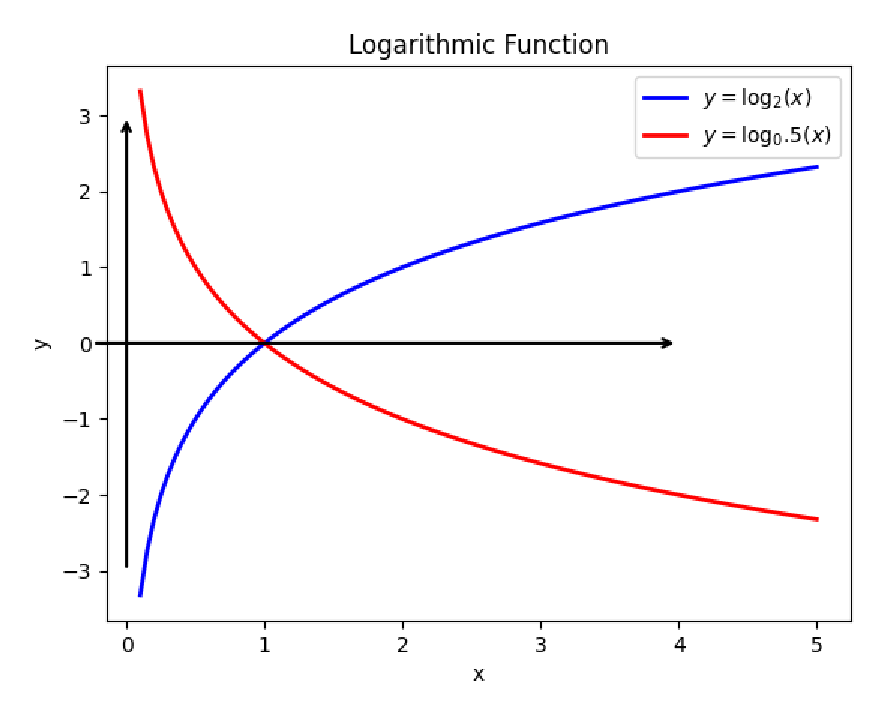
\includegraphics[width=
        0.6 \linewidth]{1.3.3.eps} \caption{对数函数图像}
\end{figure}
\subsubsection{解析式}
$$
    \boxed{y=2x}
$$